\section{Dedicated Detectors for LLPs}
\subsection{Introduction}

Some boilerplate about how, in cases of ultra-low-mass particles, ultra-long lifetimes, or unusual LLP charged, it is hard to trigger on and/or reconstruct the events in the main ATLAS, CMS, and LHCb detectors. This has led to new proposals and experiments to look for LLPs in new regimes that are otherwise inaccessible at the LHC. These experiments provide the best sensitivity to new millicharged LLPs, magnetic monopoles, and other models such as Higgs-portal hidden sectors, dark photons, and Majorana neutrinos.


\subsection{A Compact Detector for Exotics at LHCb (CODEX-b)}
\label{sec:CODEX-b}

As discussed elsewhere in the white paper, LLPs are theoretically well motivated and come in wide range of masses and lifetimes. ATLAS and CMS have excellent sensitivity for fairly high mass LLP's, regardless of their lifetime  (see e.g.~\cite{CMS:2016ybj,Aaboud:2016dgf,CMS-PAS-EXO-16-003,ATLAS-CONF-2016-103}). Low mass and/or softer final states are more challenging due to both background and triggering limitations. In the short lifetime regime, for $c\tau$ of the scale of the VELO, LHCb has sensitivity to somewhat lower masses and can trigger on softer muonic final states, generating complementary reach provided the LLP has a significant branching ratio to muons~\cite{Aaij:2017mic,Aaij:2016xmb,Aaij:2016isa,Aaij:2015ica,Aaij:2014nma}. Finally the low mass/soft final states with rather long lifetimes are challenging for all three experiments. These signatures can be covered partially by NA62~\cite{NA62:2017rwk} operating in beam dump mode, or by SHiP~\cite{Alekhin:2015byh}, or by dedicated LHC experiments like MATHUSLA~\cite{Chou:2016lxi}, FASER~\cite{Feng:2017uoz} or CODEX-b \cite{Gligorov:2017nwh}. Of these options, only MATHUSLA and CODEX-b could gather a large sample Higgs bosons.



The CODEX-b proposal involves housing a (sub)detector in the LHCb cavern in a space approximately $25$\,m from the interaction point (IP8), behind the 3m thick concrete UXA shield wall. This space is presently occupied by the LHCb data acquisition, but will become available pre-Run 3 once it is relocated to the surface. The layout of the cavern is shown in Fig.~\ref{fig:LHCbCav}, with the location of CODEX-b overlaid. 
%In particular the LHCb data acquisition system is currently housed behind the 3m thick concrete UXA shield, but will be moved to the surface during the pre-run 3 upgrade. 
The nominal CODEX-b configuration features a $10$$\times10$$\times10$\,m volume instrumented with RPC tracking layers or other off-the-shelf tracking technology, as well as roughly $25$ interaction lengths of shielding near IP8 -- e.g. $4.5$\,m of Pb --  to suppress primary and secondary $K_L$, neutron and other hadronic backgrounds. This shield requires an active muon veto with an efficiency of $\mathcal{O}(10^{-5})$, in order to reject muon or other charged particle induced backgrounds in the downstream parts of the shield: The veto is located several metres within the shield such that neutral particle induced backgrounds remain suppressed. We refer to Ref.~\cite{Gligorov:2017nwh} for a study of a proof-of-concept  example detector layout and corresponding tracking efficiency, as well as a detailed study of the backgrounds.
% It should be emphasized that for the purpose of demonstrating reach, tracking efficiencies and background control, Ref.~\cite{Gligorov:2017nwh} studied a particular proof-of-concept implementation for CODEX-b. 
More ambitious technologies, including calorimetry, precision time-of-flight, or integration into the LHCb readout may also be feasible.

\begin{figure}[t]\centering
	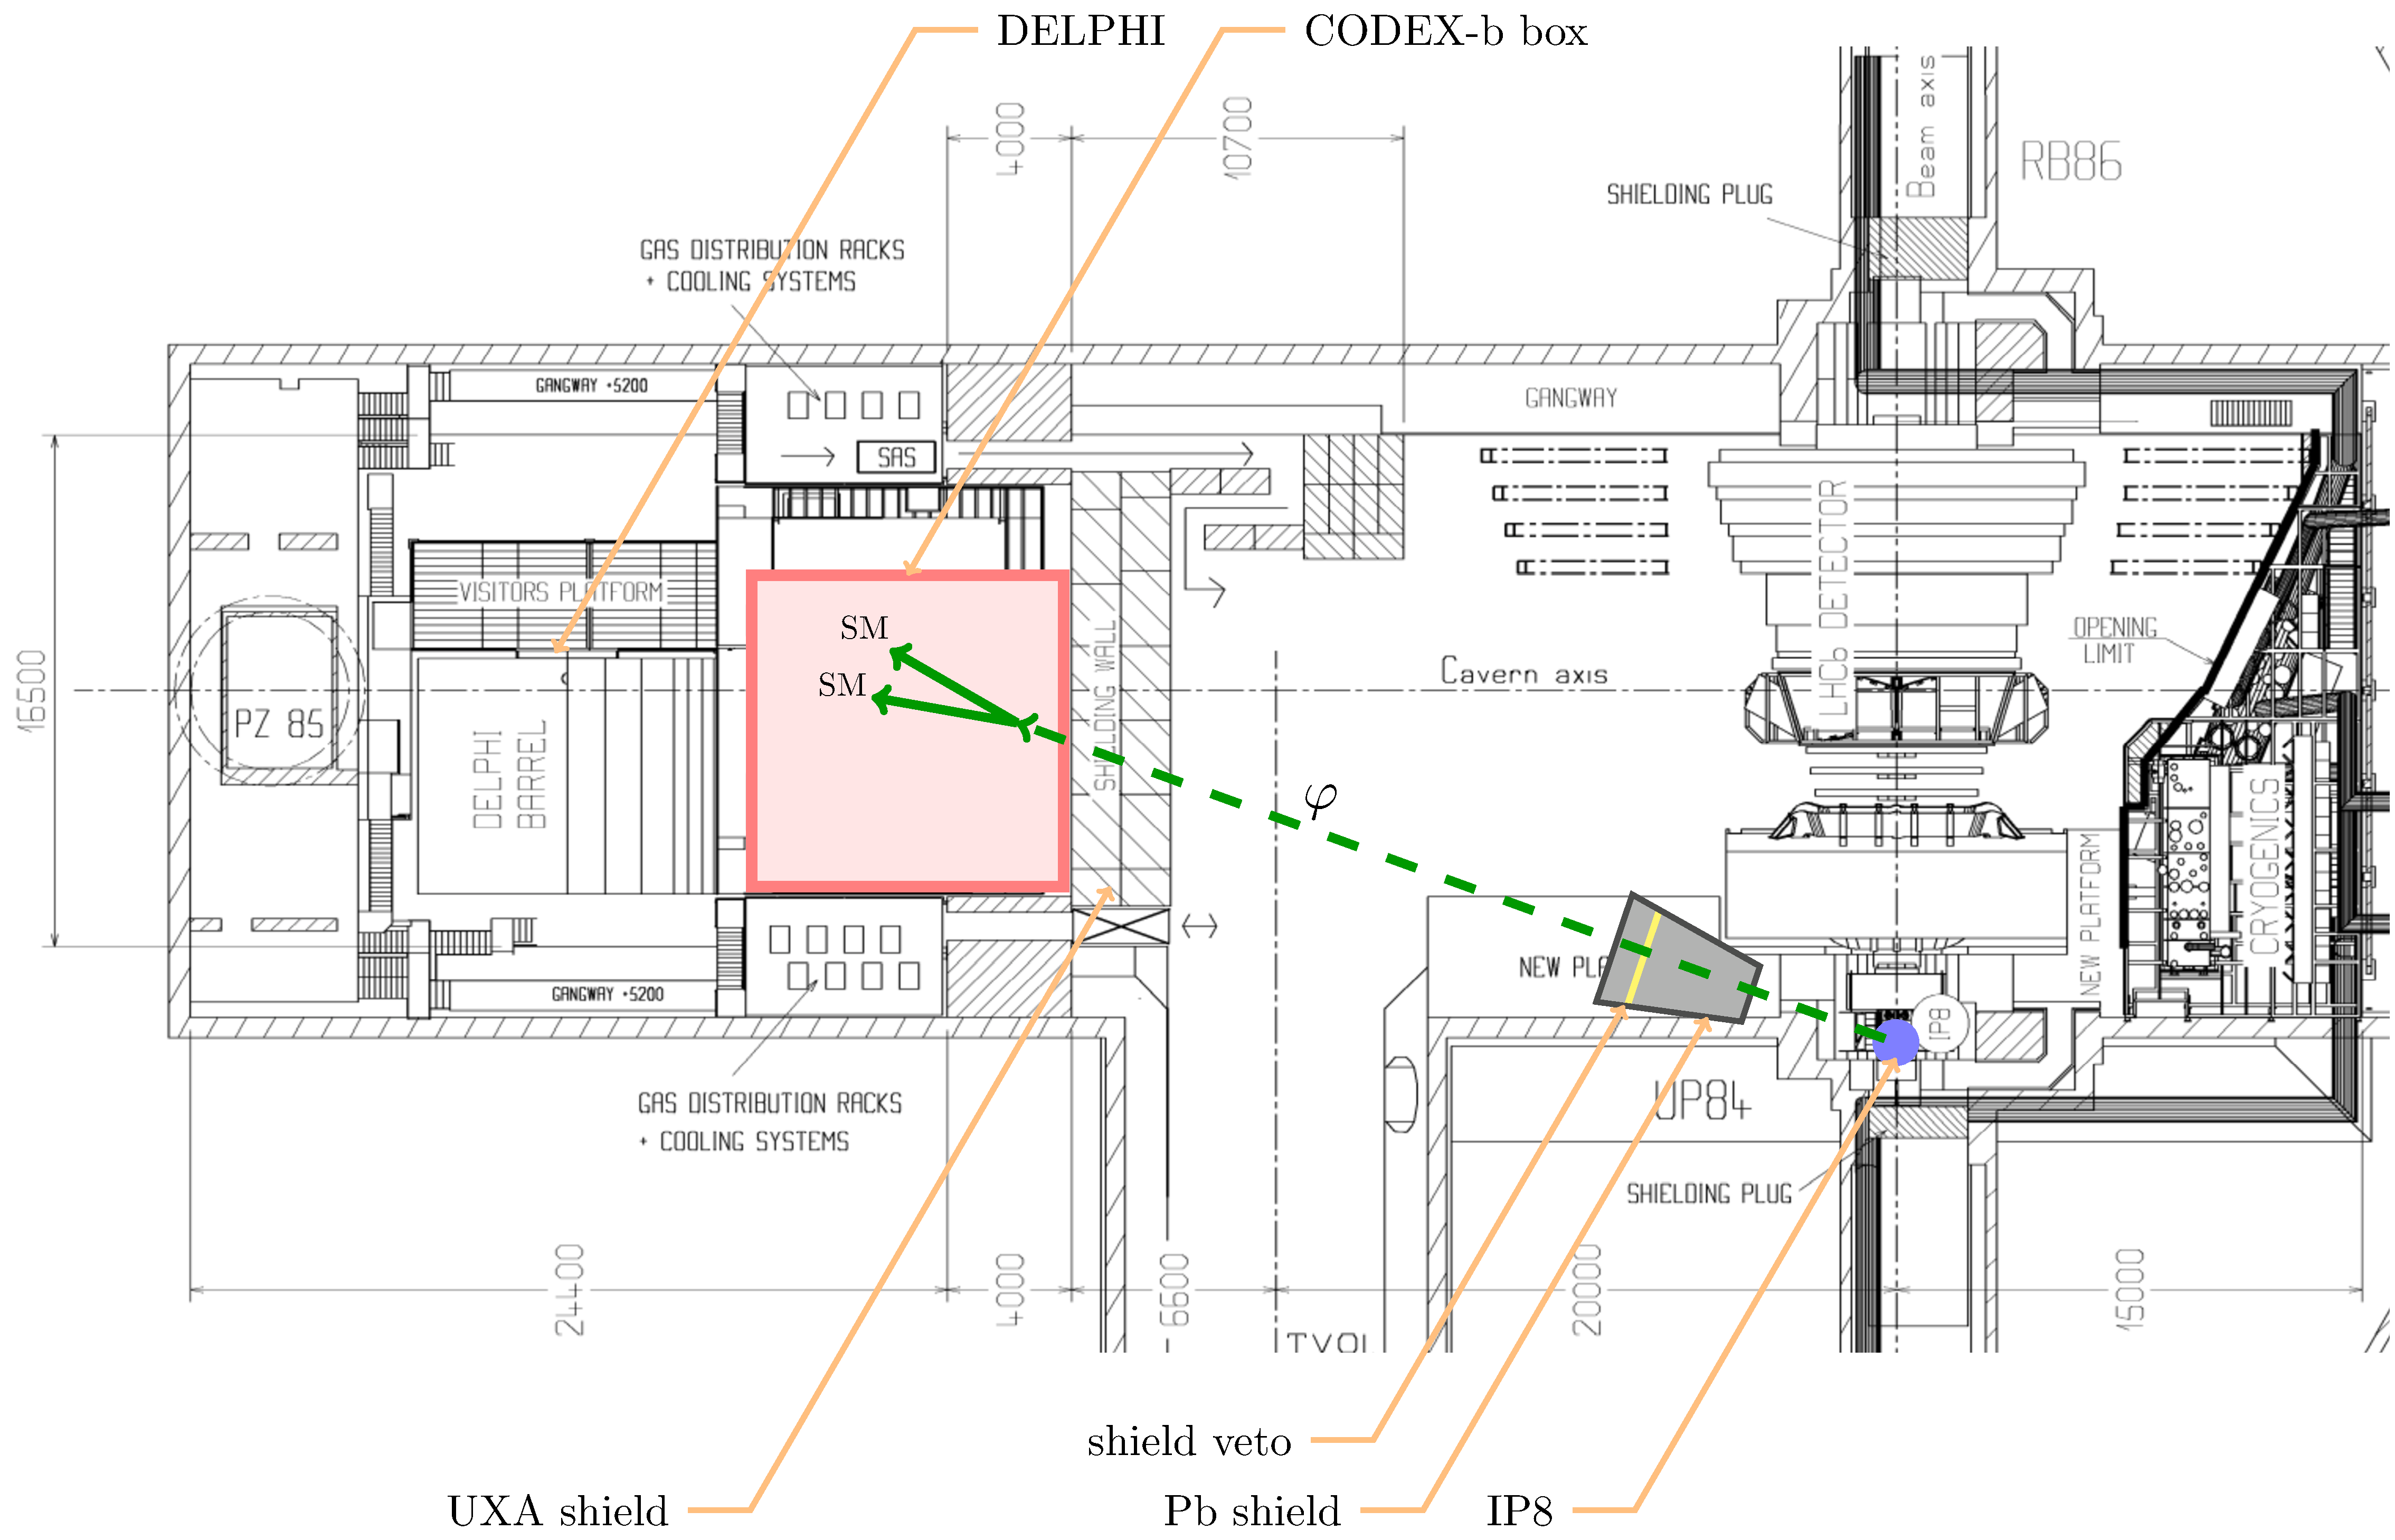
\includegraphics[width = 0.75\linewidth]{plots/LHCbCavern}
	\caption{Layout of the LHCb experimental cavern UX85 at point 8 of the LHC~\cite{cavern}, overlaid with the proposed CODEX-b location.} 
	\label{fig:LHCbCav}
\end{figure}

For the purposes of this white paper, we quantify the reach of CODEX-b for two benchmark models:
% (i) A light scalar which mixes with the Higgs and a (ii) a dark photon which is primarily produced through an exotic Higgs decay.
First we consider light scalar field, $\X$, that mixes with the SM Higgs boson. If $m_\X\lesssim$ 5 GeV, the production mode is primarily through 
inclusive $b \rightarrow s \X$ decays~\cite{Willey:1982dk,Chivukula:1988lo,Grinstein:1988yu}. The LLP $\X$ subsequently decays back to SM fermions through the same Higgs portal. The reach in terms of $m_\X$ and the mixing angle $s_\theta$ is shown in the left-hand panel of Fig.~\ref{fig:ThVM}. CODEX-b significantly extends the projected reach of LHCb using only VELO-based displaced vertex reconstruction, and covers part of the projected parameter of SHiP~\cite{Lanfranchi:2243034} and MATHUSLA  \cite{Evans:2017lvd}. Studies of the potential LHCb reach to longer lifetimes using downstream tracking are ongoing~\cite{Sierra:2017tw,Aaij:2244312}. The right-hand panel of Fig.~\ref{fig:ThVM} indicates the reach for more general models, where the lifetime and production rate of $\X$ are unrelated.


\begin{figure}[t]\centering
	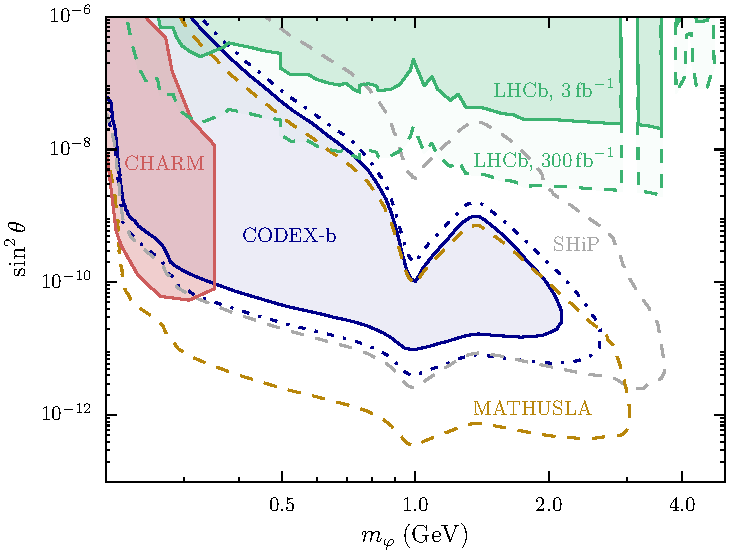
\includegraphics[height =  5cm]{plots/moneyplot_whitepaper.pdf}\hspace{2cm}
	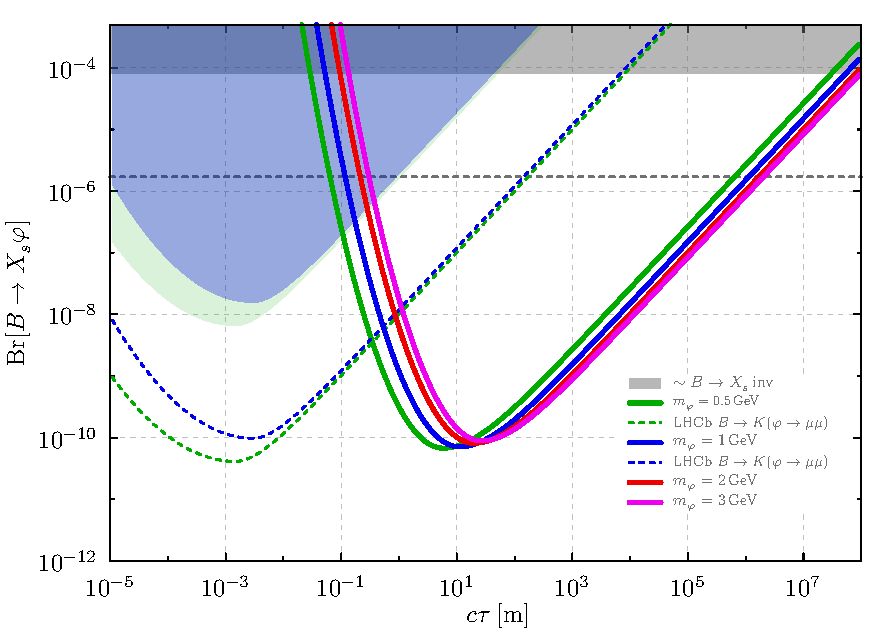
\includegraphics[height = 5cm]{plots/cTauB}
	\caption{\emph{Left:} CODEX-b reach for $B\rightarrow X_s\X$ in the $s^2_\theta$--$m_\X$ plane. Solid (dot-dashed) line assumes $\mathcal{L} = 300\, \text{fb}^{-1}$ ($\mathcal{L} = 1\, \text{ab}^{-1}$).
	\emph{Right:} Inclusive CODEX-b $B \to X_s \X$ reach (solid lines). The shaded regions (dashed lines) indicate current LHCb limits (300$\,$fb$^{-1}$ projection) from $B \to K(\X \to \mu\mu)$, rescaled to the inclusive process and assuming $\text{Br}[\X \to \mu\mu] \simeq 30\%$  and $10\%$ for $m_\X = 0.5$~GeV and $1$\,GeV, respectively. Gray shading and dashed line indicate respectively the approximate current~\cite{PDG:2016} and Belle II projected~\cite{BelleIIreport} limits from $B \to K^{(*)}\nu\bar\nu$ precision measurements.	
	} 
	\label{fig:ThVM}
\end{figure}

For our second benchmark, we consider a dark boson, $\gd$, produced through the exotic Higgs decay $h\rightarrow\gd\gd$. For concreteness we take $\gd$ to be a spin one field which can decay through mixing with the Standard Model photon~\cite{Schabinger:2005ei,Gopalakrishna:2008dv,Curtin:2014cca,Strassler:2008bv}.  In this benchmark, the production and decay are therefore controlled by different portals. The projected reach is shown in Fig.~\ref{fig:HXX}, overlaid with the reach of ATLAS \cite{Coccaro:2016lnz,ATLAS-CONF-2016-042} and MATHUSLA \cite{Chou:2016lxi}. In particular at low $\gamma_d$ masses, CODEX-b complements and significantly extends the reach of ATLAS and CMS.




\begin{figure}[t]\centering
	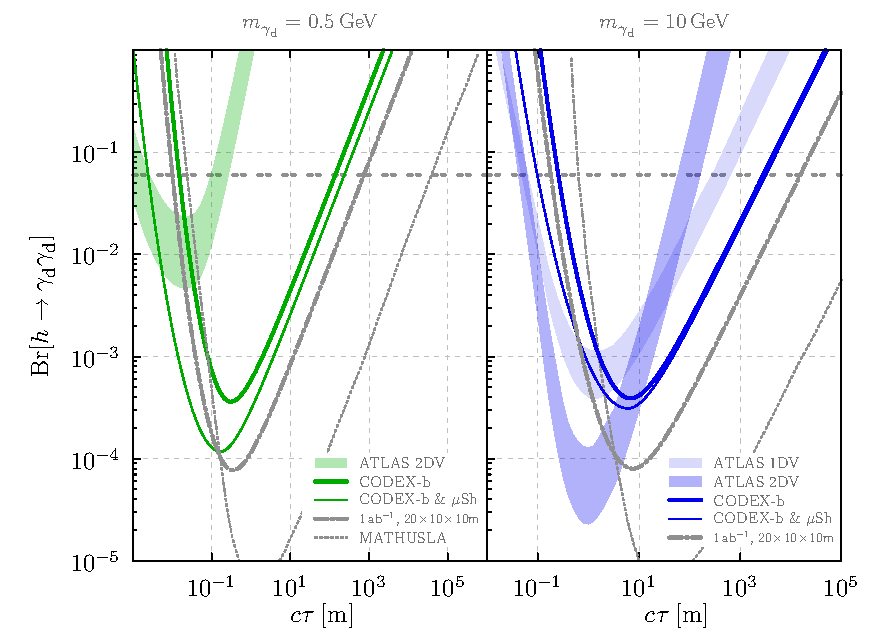
\includegraphics[height =  6cm]{plots/cTau_panel}
	\caption{Higgs decay to dark photon reach with and without the muon shadow (`$\mu$Sh'). The $\gd \to \mu\mu$ branching ratio is taken from $e^+e^-$ data~\cite{Meade:2009rb}. Also included is the optimistic CODEX-b reach with $\mathcal{L} = 1$\,ab$^{-1}$ and a larger volume, assuming DELPHI is removed. }
	\label{fig:HXX}
\end{figure}

\subsection{The ForwArd Search ExpeRiment (FASER)}
\label{sec:FASER}

\noindent {\bf Contributors:}~Jonathan L.~Feng, Iftah Galon, Felix Kling, Sebastian Trojanowski\\

\subsubsection{Introduction}
\label{sec:FASERintroduction}


If new long-lived particles are light compared to the weak scale and very weakly coupled, the focus at the LHC on searches for new particles at high $p_T$ may be completely misguided.  In contrast to TeV-scale particles, which are produced more or less isotropically, light particles with masses in the MeV-GeV range are dominantly produced at low $p_T$.  In addition, because the new particles are extremely weakly coupled, very large standard model event rates are required to discover the rare new physics events.  These rates are not available at high $p_T$, but they are available at low $p_T$: at the 13 TeV LHC, the total inelastic $pp$ scattering cross section is $\sigma_{\text{inel}}(13~\text{TeV}) \approx 75~\text{mb}$~\cite{Aaboud:2016mmw, VanHaevermaet:2016gnh}, with most of it in the very forward direction. This implies
\begin{equation}
N_{\text{inel}} \approx 2.3 \times 10^{16} \ (2.3 \times 10^{17})
\label{eq:ppcollisions}
\end{equation}
inelastic $pp$ scattering events for an integrated luminosity of $300~\text{fb}^{-1}$ at the LHC ($3~\text{ab}^{-1}$ at the HL-LHC).  Even extremely weakly-coupled new particles may therefore be produced in sufficient numbers in the very forward region.  Due to their weak coupling to the SM, such particles are typically long lived and travel a macroscopic distance before decaying back into SM particles.  Moreover, such particles may be highly collimated.  For example, new particles that are produced in pion ($B$-meson) decays are typically produced within angles of $\theta \sim \Lambda_{\text{QCD}} / E$ ($m_B / E$) of the beam-collision axis, where $E$ is the energy of the particle.  For $E \sim \text{TeV}$, this implies that even $\sim 500~\text{m}$ downstream, such particles have only spread out $\sim 10~\text{cm} - 1~\text{m}$ in the transverse plane.  A small and inexpensive detector placed in the very forward region may therefore be capable of extremely sensitive searches to LLPs, provided a suitable location can be found and the signal can be differentiated from the SM background. 

FASER~\cite{Feng:2017uoz,Feng:2017vli,Kling:2018wct}, the ForwArd Search ExpeRiment, is an experiment designed to take advantage of this opportunity.  It is a small detector, with volume $\sim 1~\text{m}^3$, that is proposed to be placed along the beam-collision axis, several hundreds of meters downstream from the ATLAS or CMS interaction point (IP). In the following, we present a promising location of FASER in Sec.~\ref{sec:FASERlocation}, discuss the properties of the signal and the required detector design in Sec.~\ref{sec:FASERDetector}, and present the new physics reach for representative models in Sec.~\ref{sec:FASERReach}. 

%%%%%%%%%%%%%%%%%%%%%%%%%%%%%%%%%%%
%%% Location                           
%%%%%%%%%%%%%%%%%%%%%%%%%%%%%%%%%%%

\subsubsection{Location}
\label{sec:FASERlocation}

As shown in Fig.~\ref{fig:Infrastructure}, FASER will be placed along the beam collision axis, several hundreds of meters downstream from the ATLAS or CMS IP after the LHC tunnel starts to curve. A particularly promising location is a few meters outside the main LHC tunnel, 480 m downstream from the ATLAS IP, in service tunnel TI18, as shown in the bottom panels of Fig.~\ref{fig:Infrastructure}. (A symmetric location on the other side of ATLAS in tunnel TI12 is also possible.) This tunnel was formerly used to connect the SPS to the LEP tunnel, but is currently empty and unused. As shown on the tunnel map in the lower left panel of Fig.~\ref{fig:Infrastructure}, the beam collision axis passes through TI18 close to where it merges with the main LHC tunnel. A more detailed study of the intersection between the beam collision axis and TI18 verifies that there exists space for FASER in the tunnel, as shown in the lower-right panel of Fig.~\ref{fig:Infrastructure}. 

In this location, FASER harnesses the enormous, previously ``wasted,'' cross section for very forward physics ($\sigma \sim \text{100 mb}$), which implies that even very weakly coupled new particles can be produced in large numbers at the LHC.  In addition, the production of LLPs at high center-of-mass energy results in long average propagation distances ($\bar{d} \sim  {\cal O}(100)~\text{m}$) and decays that are far beyond the main LHC infrastructure in regions where the backgrounds are expected to be negligible. 

%%%%%%%%%%%%%%%%%%%%
\begin{figure}[t]
\centering
\includegraphics[width=0.99\textwidth]{figures/faser/Infrastructure.pdf} 
\caption{Proposed location for FASER.  Top panel: A schematic drawing of the LHC and the very forward infrastructure downstream from the ATLAS and CMS interaction points; FASER is to be located 480 m from the IP, after the LHC ring starts to curve. Bottom panels: a map of the tunnel including the beam collision axis (left), a photo of this location (center), and a diagram showing the intersection of the beam collision axis with tunnel TI18 (right). We thank Francesco Cerutti, Paolo Fessia, Mike Lamont, and their groups for providing the photo and diagrams. 
} 
\label{fig:Infrastructure}
\end{figure}
%%%%%%%%%%%%%%%%%%%%

%%%%%%%%%%%%%%%%%%%%%%%%%%%%%%%%%%%
%%% Detector                           
%%%%%%%%%%%%%%%%%%%%%%%%%%%%%%%%%%%

\subsubsection{Signals, Detector Design and Backgrounds}
\label{sec:FASERDetector}

FASER will search for LLPs that are produced at or close to the IP, move along the beam collision axis, and decay within the volume of FASER into visible decay products
\begin{equation}
  p p  \to \text{LLP} +X, \quad  \text{LLP travels} \ \sim 480~\text{m}, \quad \text{LLP} \to \text{charged tracks} + X .
\end{equation}
LLPs produced in the very forward region of the beam collision axis typically have very high energies $E~\sim~\text{TeV}$. Although the identity of the LLP decay products depends on the mass of the LLP and the concrete new-physics model, a characteristic LLP decay signature is expected of two or more stable charged particles, such as electrons, muons or pions. This leads to a striking signature at FASER: two oppositely charged tracks with very high energy that emanate from a vertex inside the detector and which have a combined momentum that points back to the IP. A measurement of individual tracks with sufficient resolution and an identification of their charges is therefore imperative if the apparatus is to make use of kinematic features to distinguish signal from background. A tracking-based technology, supplemented by a magnet and possibly a calorimeter to allow for  energy measurements, will be the key components of FASER. 

The natural (rock) and LHC infrastructure (magnets and absorbers) shielding eliminates most potential background processes. The remaining backgrounds are expected to be mostly induced by infrastructure, mainly from collisions of the beam halo with the beam pipe near the detector and subsequent showers. Such backgrounds can be distinguished from the signal based on their different kinematic features, such as energy, direction, and track multiplicity. A further background reduction can be achieved by a scintillating veto layer that would surround the detector. Additional backgrounds from neutrino interactions within the detector are small and generally have different kinematics from signal.

A realistic background estimation for FASER poses a challenge and can best be performed with dedicated simulations, or better yet, from the experimental data themselves. A thorough such analysis using FLUKA, taking into account the exact layout of the LHC tunnels and models of radiation-matter interactions, is currently underway. 

%%%%%%%%%%%%%%%%%%%%%%%%%%%%%%%%%%%
%%% Reach                           
%%%%%%%%%%%%%%%%%%%%%%%%%%%%%%%%%%%

\subsubsection{New Physics Discovery Potential}
\label{sec:FASERReach}

%%%%%%%%%%%%%%%%%%%%
\begin{figure}[t]
\centering
\includegraphics[width=0.32\textwidth]{figures/faser/Reach_DarkPhoton.pdf} 
\includegraphics[width=0.32\textwidth]{figures/faser/Reach_DarkHiggs.pdf} 
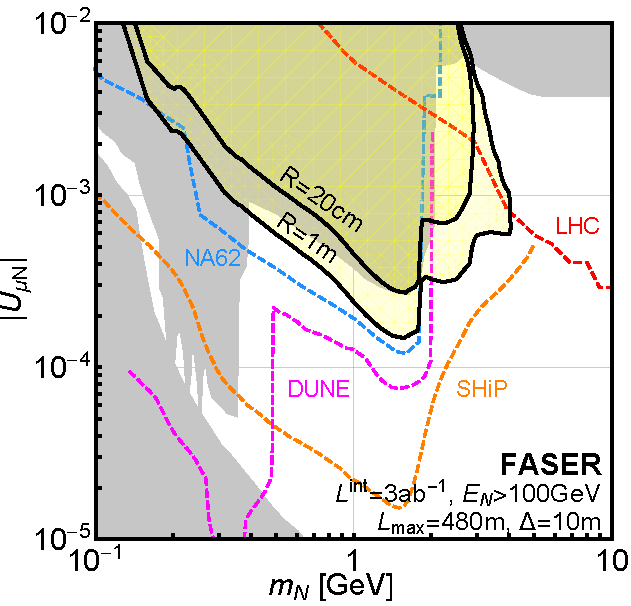
\includegraphics[width=0.32\textwidth]{figures/faser/Reach_HNL.pdf} 
\caption{
Projected FASER exclusion reach for dark photons (left), dark Higgs bosons (center), and HNLs (right) parameter space in the corresponding coupling vs. mass plane. The gray shaded regions are excluded by current experimental bounds, and the colored contours represent projected future sensitivities of other proposed experiments that search for LLPs~\cite{Alekhin:2015byh, Gardner:2015wea, Ilten:2015hya, Ilten:2016tkc, Moreno:2013mja, Chou:2016lxi, Evans:2017lvd, Gligorov:2017nwh, Adams:2013qkq, Drewes:2018gkc, Izaguirre:2015pga}.
}
\label{fig:Reach}
\end{figure}
%%%%%%%%%%%%%%%%%%%%

In previous work, we studied FASER's potential to detect dark photons~\cite{Feng:2017uoz}, dark Higgs bosons~\cite{Feng:2017vli}, and heavy neutral leptons (HNLs)~\cite{Kling:2018wct}. Combined, these studies established the significant potential for FASER to extend the LHC's discovery reach in models with renormalizable portals, where the new physics couples to the SM through dimension-4 interactions:
\begin{eqnarray}
\mathcal{L} &\subset& \epsilon F^{\mu\nu} F_{\mu\nu}^{'} \ \ \text{(dark photon)},\\
\mathcal{L} &\subset& \theta |H|^2 \phi^2  \ \ \text{(dark Higgs)},\\
\mathcal{L} &\subset& y L H N  \ \ \text{(HNL)}  \ .
\end{eqnarray}
The physics reach at FASER for these models is shown in Fig.~\ref{fig:Reach}. Here we assume that backgrounds can be reduced to negligible levels. The gray-shaded regions of parameter space have already been excluded by previous experiments. For comparison we also show the projected reaches of other proposed experiments that search for long-lived particles. 

Dark photons (left) are mainly produced in the decay of light mesons or via dark bremsstrahlung and are therefore very collimated around the beam collision axis. Already a very small detector with radius $R=20~\text{cm}$ and length $\Delta=3~\text{m}$ is able to probe large and unconstrained regions of parameter space, making dark photons an ideal short-term goal for FASER. In contrast, dark Higgs bosons and HNLs define a good long-term physics goal. They are both mainly produced in heavy-meson decays, leading to a larger spread around the beam collision axis. A larger, but still relatively small, detector with $R\sim 1~\text{m}$ is then required to exploit the full potential of FASER. 

Note that FASER's physics potential is not restricted to the models mentioned above. It has been shown that FASER can probe flavor-specific scalar mediators~\cite{Batell:2017kty}, neutralinos~\cite{Helo:2018qej}, and $U(1)_{B-L}$-gauge bosons~\cite{Bauer:2018onh}. Additionally, a study for FASER's potential to discover axion-like particles has recently been completed~\cite{Feng:2018pew}, while studies for inelastic dark matter and strongly interacting massive particles~\cite{Berlin:inprep} are underway. 


\subsection{The MATHUSLA Experiment}
\label{sec:MATHUSLA}

\noindent {\bf Contributors:}~Cristiano Alpigiani, David Curtin, Henry Lubatti, Charlie Young \\

The basic motivation for the MATHUSLA (MAssive Timing Hodoscope for Ultra-Stable neutraL pArticles) detector~\cite{Chou:2016lxi} is the search for LLPs with lifetimes much greater than the size of the LHC main detectors, $c \tau \gg 100$ m.
%
Any detector that can be reasonably constructed could only catch a small fraction of such LLPs decaying inside of its volume.
%
Even with potentially large LLP production rates at the LHC, suppression of backgrounds is  therefore crucial for discovery. 

For LLP searches with high-energy or lepton-containing final states, the spectacular  nature of displaced-vertex (DV) signals leads to very low backgrounds in searches at LHC detectors such as ATLAS or CMS.
%
Any other class of LLP signature suffers from backgrounds and triggering limitations that can be  significant. This greatly curtails the main detectors' ability to discover LLPs with very long lifetimes. 

To address this broad blind spot of existing detectors, 
MATHUSLA is proposed to be a large, relatively simple surface detector that can robustly reconstruct DVs with good timing resolution. 
%
This gives MATHUSLA a similar geometric acceptance to LLP decays in the long-lifetime limit as the main detectors, while providing shielding from QCD backgrounds and sufficient tracking to reject ubiquitous cosmic rays (CRs). 
%
As a result, MATHUSLA is able to detect LLPs produced with $\sim1$ pb cross sections at the HL-LHC with lifetimes near lifetimes of $\sim 0.1$ s, which is generally the limit imposed by Big-Bang Nucleosynthesis (BBN).


The simplified detector design for MATHUSLA is shown in Fig.~\ref{f.mathuslalayout}.
%
The main component of the detector is a tracker array situated above an air-filled decay volume that is 20 m tall and $200\,\,\mathrm{m} \times 200\,\,\mathrm{m}$ in area. The tracker should have on the order of 5 planes to provide robust tracking with $\sim$ ns, cm timing and spatial resolution, respectively.
%
The current MATHUSLA design employs proven and relatively cheap technologies to allow for MATHUSLA's construction in time for the HL-LHC upgrade. Therefore, the trackers are envisioned to be implemented with Resistive Plate Chambers (RPCs), which have been used for very large area experiments in the past~\cite{Aielli:2006cj, Iuppa:2015hna}, while plastic scintillators provide the surrounding veto.  


\begin{figure}
\begin{center}
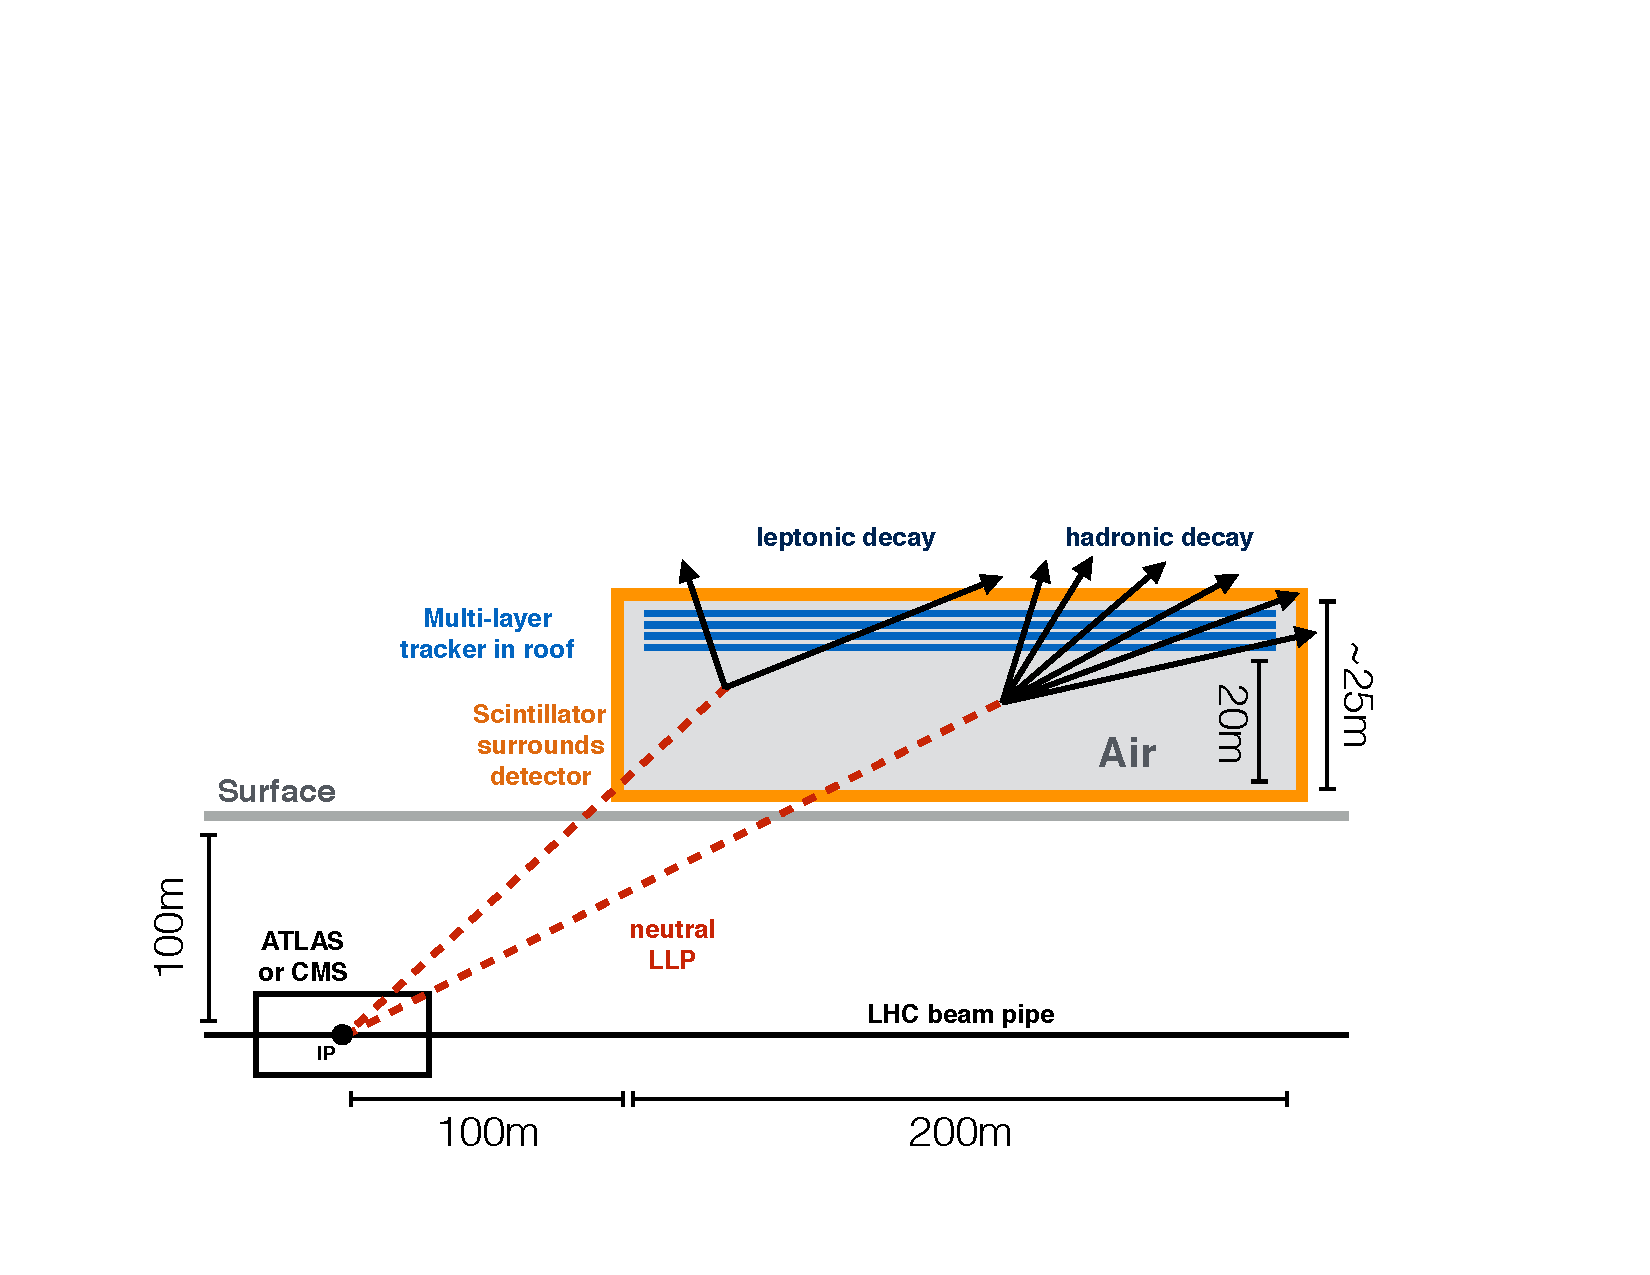
\includegraphics[width=0.6\textwidth]{figures/mathusla/3_mathusla.pdf}
\end{center}
\caption{
Simplified MATHUSLA detector layout showing the position of the $200\,\,\mathrm{m} \times 200\,\,\mathrm{m} \times 20\,\,\mathrm{m}$ LLP decay volume.
}
\label{f.mathuslalayout}
\end{figure}


This minimal design has been shown to be capable of measuring the LLP boost  on an event-by-event basis~\cite{Curtin:2017izq} using  the geometry of the LLP visible decay products. Final-state multiplicity provides a straightforward discriminant between hadronic and electromagnetic decays. Additional particle identification capability, as well as detection of final-state photons, might be possible by inserting an additional material layer between tracking layers to induce an electromagnetic shower that can be used to distinguish electrons, photons and muons.

%%%%%%%%%%%%%%%%%%%%

As argued in Ref.~\cite{Chou:2016lxi}, MATHUSLA could search for LLPs decaying into  charged particles with little or no backgrounds. 
%
Fig.~\ref{f.mathuslalayout} schematically shows the two main MATHUSLA signals, LLPs decaying into at least two charged leptons, or into jets that contain $\mathcal{O}(10)$ charged hadrons~\cite{Curtin:2017izq}. 
% summary of signal requirements
In 50-90\% of leptonic decays and practically 100\% of hadronic decays~\cite{Curtin:2017izq}, 2 or more charged partices hit the ceiling due to the LLP boost and are recorded by the tracker. The charged particle trajectories can be fitted to reconstruct a DV.
%
Unlike most analyses in the main detectors, these DVs must satisfy the additional stringent requirement that all trajectories coincide in time at the DV. 
%
The scintillator is used as a veto to ensure that the charged particles originate at the DV:~there can be no hits along the line between the vertex and the LHC main interaction point (IP), nor along the lines obtained by extrapolating the individual charged particle trajectories backwards.
%
These exhaustive geometric and timing requirements make it extremely difficult for backgrounds to fake the LLP signal.
%
Cosmic rays can be rejected since they travel in the wrong direction (as well as occurring mostly in cosmic ray showers with extremely highly correlated particle multiplicity in the detector).  
%
Muons from the LHC collision do not satisfy the DV signal requirement. The rare occasions in which muons scatter inside the decay volume can be vetoed with the scintillators. 
%
Finally, neutrinos from cosmic rays and LHC collisions can scatter in the decay volume and produce displaced vertices, but those can also be rejected with geometric and timing requirements. 
We refer the reader to Ref.~\cite{Chou:2016lxi} for more details. 
%
More comprehensive studies of these backgrounds and their rejection strategies, including full simulations, are currently in progress. 



\begin{figure}
\begin{center}
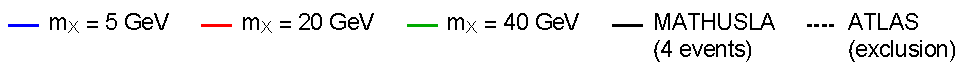
\includegraphics[width=0.8\textwidth]{figures/mathusla/limitlegend_14TeV}
\\
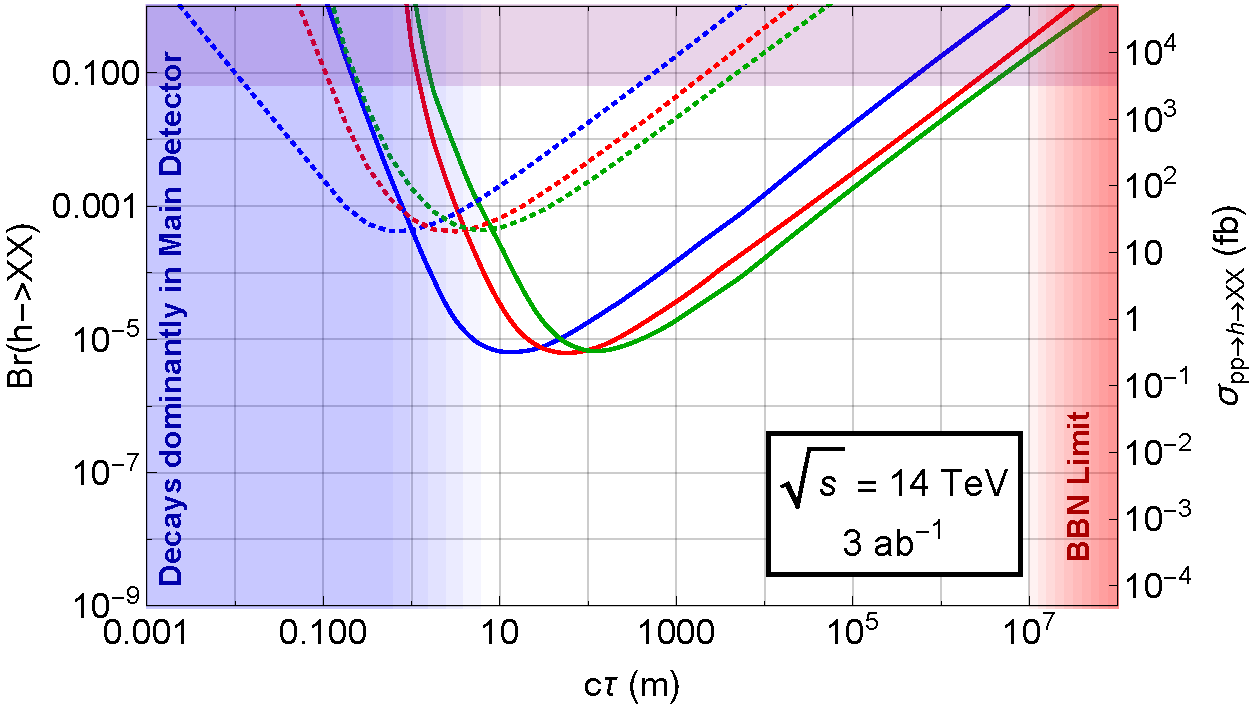
\includegraphics[width=0.8\textwidth]{figures/mathusla/LLPlimits_14TeV_forpaper}
\end{center}
\caption{
Sensitivity of MATHUSLA to hadronically decaying LLPs produced in exotic Higgs decays (solid lines correspond to 4 decays in the detector)~\cite{Chou:2016lxi}. The dotted lines are the most optimistic ATLAS projection, using a very inclusive search for a single DV in the muon chamber~\cite{Coccaro:2016lnz}.
}
\label{f.mathuslahiggs}
\end{figure}

An important general class of signals are LLPs with masses $\lesssim 100 \gev$ that decay hadronically and are produced without other highly visible signals like high MET or high-energy leptons. 
%
MATHULSLA can improve the sensitivity to these LLP production cross sections by a factor of $\sim 10^3$ compared to searches with the main detectors alone. 
%
This is illustrated in Fig.~\ref{f.mathuslahiggs}, which shows MATHUSLA's sensitivity to hadronically decaying LLPs produced in exotic Higgs decays~\cite{Chou:2016lxi} compared to an optimistic  projection for searches for a single DV in the ATLAS muon spectrometer~\cite{Coccaro:2016lnz}. 
%
For branching ratios of $\sim 10\%$, the BBN lifetime limit~\cite{Fradette:2017sdd} can be probed. 


Apart from reaching the BBN ``ceiling'' of LLP parameter space, MATHUSLA extends the power of other LHC measurements. 
If a $\sim 10\%$ invisible branching ratio for the Higgs was detected via coupling measurements at the HL-LHC, the absence of a MATHUSLA signal would lend strong support to the interpretation that the Higgs decayed to a stable component of dark matter. 


% sensitivity from higgs decays
% mass threshold: boost
Beyond LLPs produced in rare Higgs decays, MATHUSLA is a general-purpose LLP detector sensitivity to a wide range of other models. Its reach for other BSM scenarios has been explored in~\cite{Co:2016fln, Dev:2016vle, Dev:2017dui, Caputo:2017pit, Evans:2017lvd, Evans:2017kti, Helo:2018qej, DAgnolo:2018wcn, Deppisch:2018eth, Jana:2018rdf}. The general physics case for MATHUSLA's construction is  made systematically in the recently released whitepaper~\cite{Curtin:2018mvb}.


It is important to point out that MATHUSLA is a very flexible detector concept that is completely scalable. 
%
The sensitivity of MATHUSLA is roughly proportional to the decay volume (which scales with surface area) and roughly independent of the precise geometry or location of the detector, as long as it is $\mathcal{O}(100 \,\,\mathrm{m})$ horizontally displaced from the IP. 
%
Therefore, a detector with smaller or larger volume than the benchmark in Fig.~\ref{f.mathuslalayout} may be implemented, depending on available space and budget. 
%
Furthermore, the detector volume can be divided into smaller, independent modules (which cooperate for triggering purposes). These can be mass-produced economically and arranged according to the requirements of the experimental site. 
%
Such a modular construction also makes it natural to upgrade (say) only one or a few modules with additional capabilities, such as higher tracking resolution for reconstruction of very low-mass LLPs below 10 MeV, or an additional material layer between the trackers for particle ID.


The MATHUSLA collaboration is currently studying such a modular design with the aim of producing a Letter-of-Intent in 2018. Crucial to this endeavor is the data from the MATHUSLA test stand, a $\sim 3 \times 3 \times 5$ m MATHUSLA-type detector that took a few days of data in the ATLAS instrument hall in 2017 and will take data for a few months in 2018. This allows local cosmic ray backgrounds to be measured, background rejection and signal reconstruction strategies to be tested, and simulation frameworks to be calibrated. 


In conclusion, the MATHUSLA detector concept calls for a dedicated LLP surface detector above ATLAS or CMS. 
%
A detector volume of $\sim 10^6\,\,\mathrm{m}^3$ gives sensitivity to LLPs near the BBN lifetime limit if they are produced with $\sim$ pb cross section. This improves LLP sensitivity, compared to the main detectors alone, by several orders of magnitude for many LLP scenarios.
%
 The detector is simple and relies on proven technology, making its construction in time for the HL-LHC upgrade feasible. Once constructed, MATHUSLA could function without modification as a detector for the HE-LHC (with increased sensitivity).
 %
 A small-scale test stand detector is already taking data at CERN, and studies are underway to finalize a detailed design for the full-scale detector.

\subsection{The MilliQan Experiment}
\label{sec:milliQan}

\noindent {\bf Contributor:}~Christopher Hill \\

MilliQan is a dedicated experiment at the LHC to search for milli-charged particles (mCP)~\cite{Ball:2016zrp, Haas:2014dda}. The MilliQan experiment is part of a general program to search for hidden sectors~\cite{Izaguirre:2015eya} and other BSM scenarios~\cite{Sher:2017wya}. As an illustrative example, we show the sensitivity of MilliQan to an extra abelian gauge field coupled to a massive Dirac fermion (``dark QED") that mixes with hypercharge through the kinetic term~\cite{Holdom:1985ag}. The result is that the new matter field is charged under hypercharge with a fractional electric charge of $\epsilon$, where $\epsilon \ll 1$. The milliQan experiment targets an unexplored part of the parameter space, namely mCP masses $0.1 \lsim \MQ \lsim 100 \gev$, for charges $Q$ at the $10^{-3}~e -10^{-1}~e$ level. 

The  experimental apparatus  is one or more scintillator detector layers of roughly 1 m$^3$ each, positioned near one of the high-luminosity interaction points of the LHC. The experimental signature consists of a few photo-electrons (PE) arising from the small ionization produced by the mCPs that travel unimpeded through material after escaping the LHC detectors.

 The milliQan experiment is planned to be sited in the PX56 Observation and Drainage gallery above the CMS underground experimental cavern. The proposed gallery is limited in space. The detector will be located in this tunnel at an optimized location that is 33~m from the CMS  interaction point (IP), behind 17~m of rock, and at an angle of 43.1 degrees from the horizontal plane. The selected location in a 3D model is shown in Figure~\ref{fig:site}. 

\begin{figure}[htp]
\centering
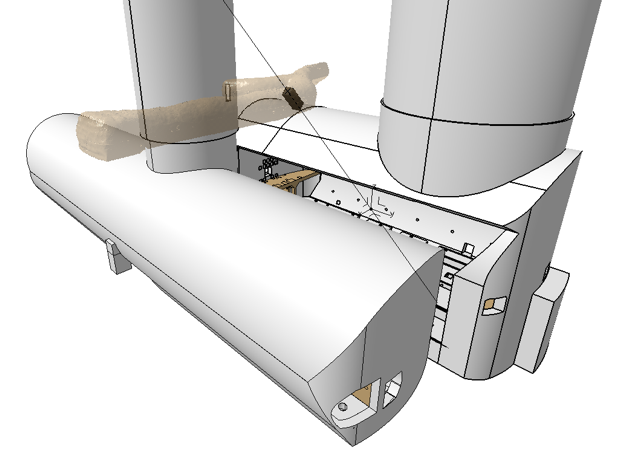
\includegraphics[width=0.6\linewidth]{figures/milliqan/site_selection_image.png}
\caption{3D model showing optimal position of milliQan within the PX56 Drainage and Observation gallery located above CMS UXC.\label{fig:site}}
\end{figure}

 The milliQan detector is a~$1~\mathrm{m}\times1~\mathrm{m}\times3~\mathrm{m}$ plastic scintillator array. The array will be oriented such that the long axis points at the nominal CMS IP. The array is subdivided into 3 sections each containing 400~$5~\mathrm{cm}\times5~\mathrm{cm}\times80~\mathrm{cm}$ scintillator bars optically coupled to high-gain photomultiplier tubes (PMTs).  The detector will be shielded from other background sources such as activity in the scintillator and environmental radiation. With an estimated detection efficiency of about 10\%, milliQan expects an average of $\mathcal{O}(1)$ PE from each attached phototube for each mCP with $Q=\mathcal{O}(10^{-3})~e$ that traverses 80~cm of plastic scintillator. The signal is a longitudinal triple-incidence of hits with one or more PEs; a triple-incidence within a 15 ns time window along longitudinally contiguous bars in each of the 3 sections is required to reduce the background from dark-current noise. Requiring triple-incidence is expected to control background to $\mathcal{O}(10)$ events per year with $N_{\rm PE}\ge 1$. The milliQan detector will self-trigger to a dedicated readout with no dead time from readout, up to rates of $\sim1$~kHz. Energy calibration will be done in situ using an $^{241}$Am source. 
 
  The dominant background is expected to come from dark-current pulses in the PMTs. Pulses from background radiation, including cosmic muons, will consist of 1000 of PEs that can be easily vetoed offline. Assuming a total background rate per PMT of $\nu_B = $500 Hz, with a time window of $(\Delta t)_{\mathrm{online}} =100$~ns, milliQan expects a double coincident trigger rate per board of 1.5~Hz. The entire detector will be read out if one board triggers and there will be 50 such boards in total. Therefore, the full background trigger rate is expected to be 75~Hz. Offline, the time window will be tightened to $(\Delta t)_{\mathrm{offline}} =15$~ns, yielding an offline background rate for a triple coincidence of $2.8\times10^{-8}$~Hz. Since there are 400 such sets, the total offline background rate is estimated to be $1.1\times10^{-5}$~Hz. With these background rates, milliQan  estimates a total of 165 (330) background events in 300 (3000)~fb$^{-1}$ of integrated luminosity. 

 The milliQan collaboration performed a full simulation of the experiment to evaluate the projected sensitivity of the experiment for various mCP electric charges and masses. The simulation was performed in two stages. In the first, they simulated the production of mCP particles via Drell-Yan, J/$\Psi$, $\Upsilon$(1S), $\Upsilon$(2S), and $\Upsilon$(3S) channels at 14 TeV center-of-mass energy. Particles produced at the IP were propagated  to the proposed experimental site described above using a map of the CMS magnetic field. The effects of multiple scattering and energy loss were included using a simplified model of the CMS detector material budget and a region of rock spanning 17~m between the CMS experimental cavern and the proposed experimental site. The number of expected mCP particles per fb$^{-1}$ of integrated luminosity incident at the detector was computed as a function of the mass of the milli-charged particle. In the second stage, milliQan calculates the signal efficiency by running the kinematic distributions of the particles at the proposed experimental site through a full {\sc Geant4} simulation of the detector; this is necessary because the small charge regime is sensitive to details such as the reflectivity, the light attenuation length, and the shape of the scintillator. These details, as well as the quantum efficiency, light-emission spectrum and the fast-time constants were modeled in {\sc Geant4} using the specifications provided by the manufacturers for the scintillator and PMTs. Combining the estimated background rates discussed above with the cross-sections, acceptances and efficiencies calculated for all masses and electric charges, the sensitivity projections of the milliQan experiment for LHC and HL-LHC are shown in Figure~\ref{fig:abc}.


\begin{figure}[h]
   \centering
   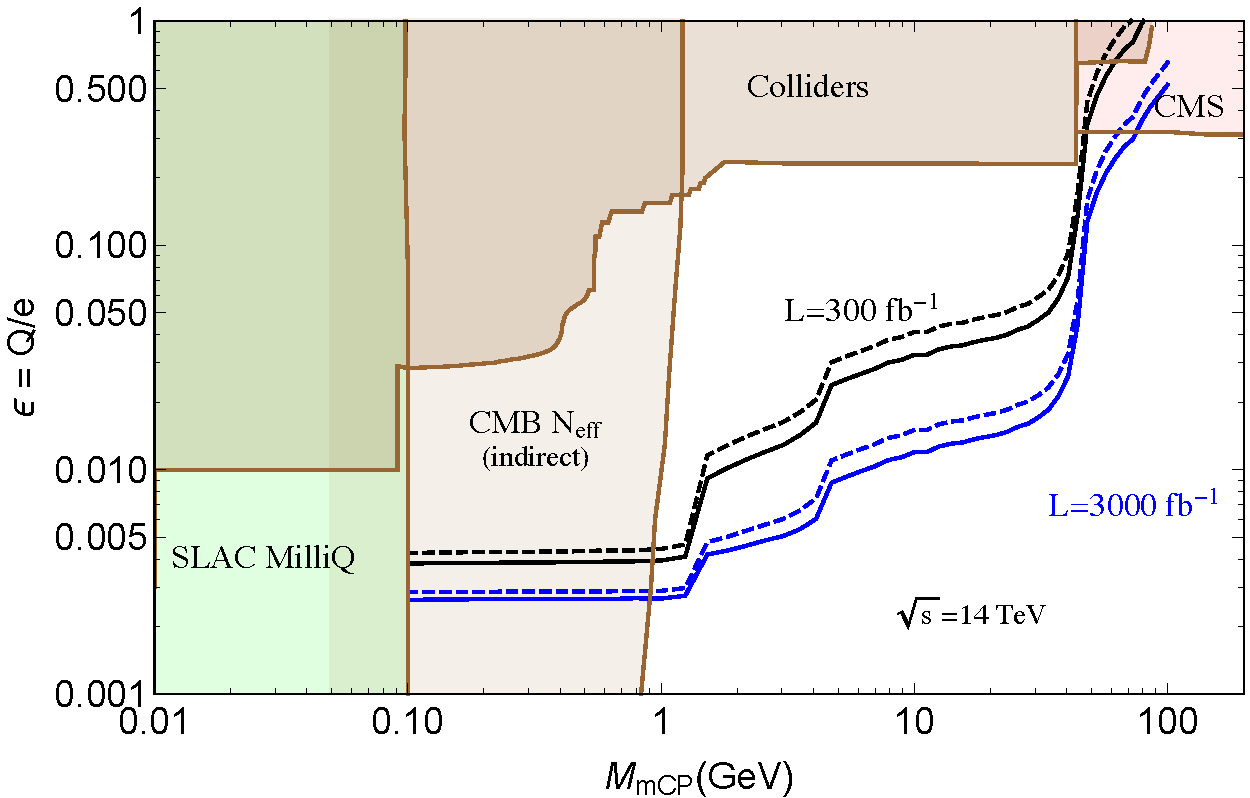
\includegraphics[width=0.6\linewidth]{figures/milliqan/exclusionplots_5b5.pdf}
   \caption{Expected sensitivity for different LHC luminosity scenarios. The black line shows the expected 95\% C.L. exclusion (solid) and $3\sigma$ sensitivity (dashed),
assuming $300~\text{fb}^{-1}$ of integrated luminosity. In blue we show the corresponding expectations for $3000~\text{fb}^{-1}$.
\label{fig:abc}}
\end{figure}

 
 A 1/100th scale ``demonstrator'' of milliQan to validate the detector concept was installed in the PX56 location at CERN in technical stop 2 of 2017 and was upgraded during the 2017--2018 year-end technical stop. This demonstrator, shown in Figure~\ref{fig:demo}, has been recording data since its installation, and expects to have first results later this year. If funding is secured, construction of the full milliQan apparatus is planned for 2019, with installation in the tunnel in 2020. 

\begin{figure}[h]
   \centering
   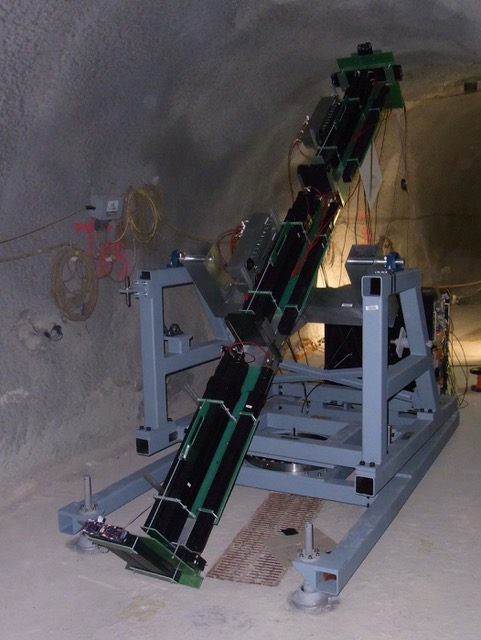
\includegraphics[width=0.5\linewidth]{figures/milliqan/RIMG0141.jpg}
   \caption{ 1/100th scale ``demonstrator'' of milliQan installed in the PX56 drainage gallery 33 m from the CMS IP.
\label{fig:demo}}
\end{figure}


\subsection{MoEDAL experiment and future developments}
\label{sec:MoEDAL}

\noindent {\bf Contributors:}~Philippe Mermod, Vasiliki A.\ Mitsou, James L.~Pinfold

\subsubsection{Introduction}\label{sc:intro}

MoEDAL (Monopole and Exotics Detector at the LHC)~\cite{Pinfold:2009oia}\footnote{For general information on the MoEDAL experiment, see: \url{http://moedal.web.cern.ch/}.} is designed to search for manifestations of new physics through highly-ionising (HI) particles in a manner complementary to ATLAS and CMS~\cite{DeRoeck:2011aa}. The main motivation for the MoEDAL experiment is to pursue the quest for magnetic monopoles at LHC energies. Nonetheless the detector is also designed to search for any massive,  long-lived, slow-moving particle~\cite{Fairbairn:2006gg,Burdin:2014xma} with single or multiple electric charges arising in many scenarios of physics beyond the Standard Model~\cite{Acharya:2014nyr}. 

%%%%%%%%%%%%%%%%%%%%%%%%%%%%%%%%%%%%%%%%%%%%%%%%%%%
%%%%%%%%%%%%%%%%%%%%%%%%%%%%%%%%%%%%%%%%%%%%%%%%%%%
\subsubsection{The MoEDAL detector}\label{sc:detector}

The MoEDAL detector~\cite{moedal} is deployed around the intersection region at the LHC Point~8 (IP8) in the LHCb Vertex Locator (VELO) cavern. A schematic view of the MoEDAL experiment is shown in Fig.~\ref{fg:moedal-lhcb}. It is a unique and largely passive detector comprising different detector technologies. 
\begin{figure}[htb]
\begin{minipage}[b]{0.55\textwidth}
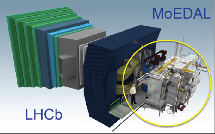
\includegraphics[width=\textwidth]{plots/moedal-detector}
\end{minipage}\hspace{0.05\textwidth}%
\begin{minipage}[b]{0.4\textwidth}
\caption{\label{fg:moedal-lhcb} A three-dimensional schematic view of the MoEDAL detector (in the yellow circle) around the LHCb VELO region at Point~8 of the LHC.}
\end{minipage} 
\end{figure}

%%%%%%%%%%%%%%%%%%%%%%%%%%%%%%%%%%%%%%%%%%%%%%%%%%%
%\subsection{Low-threshold nuclear track detectors}\label{sc:ndt}
\subsection{Nuclear track detectors}\label{sc:ndt}

The main sub-detector system is made of a large array of CR39$^{\tiny{\textregistered}}$,  Makrofol$^{\tiny{\textregistered}}$ and Lexan$^{\tiny{\textregistered}}$ nuclear track detector (NTD) stacks surrounding the intersection area. The passage of a HI particle through the plastic detector is marked by an invisible damage zone along the trajectory. The damage zone is revealed as a cone-shaped etch-pit when the plastic detector is chemically etched. Then the sheets of plastics are scanned looking for aligned etch pits in multiple sheets. The MoEDAL NTDs have a threshold of $Z/\beta\sim5$, where $Z$ is the charge and $\beta=v/c$ the velocity of the incident particle. 

Another type of NTD installed is the Very High Charge Catcher ($Z/\beta\sim50$). It consists of two flexible low-mass stacks of Makrofol$^{\tiny{\textregistered}}$, deployed in the LHCb acceptance between RICH1 and the Trigger Tracker. It is the only NTD (partly) covering the forward region, adding only $\sim0.5\%$ to the LHCb material budget while enhancing considerably the overall geometrical coverage of MoEDAL.

%%%%%%%%%%%%%%%%%%%%%%%%%%%%%%%%%%%%%%%%%%%%%%%%%%%
\subsection{Magnetic trappers}\label{sc:mmt}

A unique feature of the MoEDAL detector is the use of paramagnetic magnetic monopole trappers (MMTs) to capture magnetically-charged HI particles. The high magnetic charge of a monopole ---being at least one Dirac charge $g_{\rm D} = 68.5 e$--- implies a strong magnetic dipole moment, which may result in strong binding of the monopole with the nuclei of the aluminium MMTs. In such a case, the presence of a trapped monopole would de detected through the induction technique by measuring the \emph{persistent current}, defined as the difference between the superconducting magnetometer currents before and after the passage of the MMT bar through the sensing coil~\cite{Joergensen:2012gy,DeRoeck:2012wua}. 

%%%%%%%%%%%%%%%%%%%%%%%%%%%%%%%%%%%%%%%%%%%%%%%%%%%
\subsection{TimePix radiation monitors}\label{sc:timepix}

The only non-passive MoEDAL sub-detector is an array of TimePix pixel devices distributed throughout the MoEDAL cavern, forming a real-time radiation monitoring system of HI beam-related backgrounds. The operation in time-over-threshold mode allows a 3D mapping of the charge spreading in the volume of the silicon sensor, thus differentiating between various particles species from mixed radiation fields and measuring their energy deposition.

%%%%%%%%%%%%%%%%%%%%%%%%%%%%%%%%%%%%%%%%%%%%%%%%%%%
%%%%%%%%%%%%%%%%%%%%%%%%%%%%%%%%%%%%%%%%%%%%%%%%%%%
\subsubsection{MoEDAL physics goals}\label{sc:mm}

The MoEDAL detector is designed to fully exploit the energy-loss mechanisms of magnetically charged particles~\cite{Dirac:1931kp,Dirac:1948um,tHooft:1974kcl,Polyakov:1974ek}  in order to optimise its potential to discover these messengers of new physics. There are various theoretical scenarios in which magnetic charge would be produced  at the LHC~\cite{Acharya:2014nyr}: (light) 't Hooft-Polyakov monopoles~\cite{tHooft:1974kcl,Polyakov:1974ek,Vento:2013jua}, electroweak monopoles~\cite{Cho:1996qd,Bae:2002bm,Cho:2012bq,Cho:2016npz,Ellis:2016glu}, global monopoles~\cite{Barriola:1989hx,Drukier:1981fq,Mazur:1990ak,Mavromatos:2016mnj} and monopolium~\cite{Dirac:1948um,Zeldovich:1978wj,Hill:1982iq,Dubrovich:2002gp}. Magnetic monopoles that carry a non-zero magnetic charge and dyons possessing both magnetic and electric charge are predicted by many theories including grand-unified and superstring theories~\cite{Rajantie:2012xh,Rajantie:2016paj,Kephart:2017esj}. 
 
A possible explanation for the non-observation of monopoles so far is Dirac's proposal~\cite{Dirac:1931kp,Dirac:1948um,Zeldovich:1978wj} that monopoles are not seen freely because they form a bound state called \emph{monopolium}~\cite{Hill:1982iq,Dubrovich:2002gp,Epele:2007ic,Epele:2008un} being confined by strong magnetic forces. Monopolium is a neutral state, difficult to detect directly at a collider detector, although its decay into two photons would give a rather clear signal for ATLAS and CMS~\cite{Epele:2016wps}. Nevertheless the LHC radiation detector systems can be used to detect final-state protons $pp\to pXp$ exiting the LHC beam vacuum chamber at locations determined by their fractional momentum losses~\cite{Kalliokoski:2016fjr}. Such technique would be appealing for detecting monopolia. 

The MoEDAL detector is also designed to search for any massive, long-lived, slow-moving particles~\cite{Fairbairn:2006gg,Burdin:2014xma} with single or multiple electric charges  arising in many scenarios of physics beyond the Standard Model. Supersymmetric long-lived particles, quirks, strangelets, Q-balls, and many others fall into this category~\cite{Acharya:2014nyr}.

%%%%%%%%%%%%%%%%%%%%%%%%%%%%%%%%%%%%%%%%%%%%%%%%%%%%%%%%%%%%%%%%%%%%%%%%%%%%%%%%%%%%%%%%%%%%%%%%%%%%%%
\subsection{Searches for monopoles in MoEDAL}\label{sc:lightsearch}

For the 2015 run at 13~TeV, the MMT consisted of 672~aluminium rods for a total mass of 222~kg that were placed 1.62~m from the IP8 LHC interaction point under the beam pipe on the side opposite to the LHCb detector. The MMT bars were analysed and no magnetic charge  $>0.5g_{\rm D}$ was detected in any of the exposed samples when passed through the ETH Zurich SQUID. Hence cross-section limits are obtained for Drell-Yan (DY) pair production of spin-1/2 and spin-0 monopoles for $1g_{\rm D}\leq|g|\leq 5g_{\rm D}$ at 13~TeV~\cite{Acharya:2016ukt,Acharya:2017cio} improving previous bounds set by MoEDAL at 8~TeV~\cite{MoEDAL:2016jlb}. However, the large monopole-photon coupling invalidates any perturbative treatment of the cross-section calculation and hence any result based on the latter is only indicative. This situation may be resolved if thermal production in heavy-ion collisions ---that does not rely on perturbation theory--- is considered~\cite{Gould:2017zwi}.
\begin{figure}[htb]
\begin{minipage}[b]{0.5\textwidth}
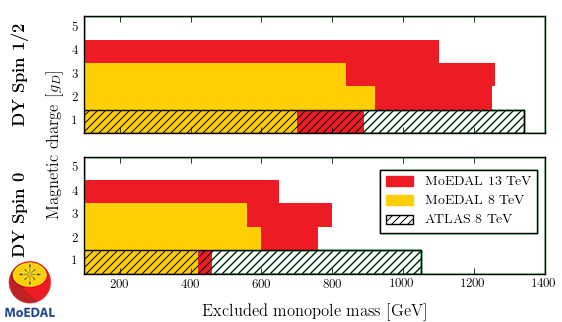
\includegraphics[width=\textwidth]{plots/exclusion3}
\caption{\label{fg:limits} Excluded monopole masses for DY production for spin-$1/2$ (top) and spin-$0$ (bottom) monopoles. The MoEDAL results obtained at 8~TeV~\cite{MoEDAL:2016jlb} and 13~TeV~\cite{Acharya:2016ukt} are superimposed on the ATLAS 8-TeV limits~\cite{Aad:2015kta}.}
\end{minipage}\hspace{0.05\textwidth}%
\begin{minipage}[b]{0.45\textwidth}
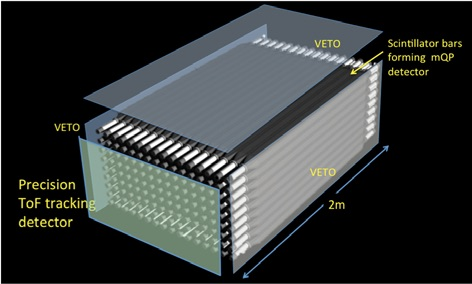
\includegraphics[width=\textwidth]{plots/mapp.jpg}
\caption{A depiction of a MAPP detector subunit. The final detector could contain up to four such units.~\cite{Pinfold:2017dot}.}
\label{fg:mapp}
\end{minipage} 
\end{figure}

Under the assumption of Drell-Yan cross sections, mass limits are derived for $g_{\rm D}\leq|g|\leq4g_{\rm D}$ at the LHC, complementing ATLAS results~\cite{Aad:2012qi,Aad:2015kta}, which placed limits for monopoles with magnetic charge $|g|\leq1.5 g_{\rm D}$, as shown in Fig.~\ref{fg:limits}. The ATLAS bounds are better that the MoEDAL ones for $|g|=1 g_{\rm D}$ due to the higher luminosity delivered in ATLAS and the loss of acceptance in MoEDAL for small magnetic charges. On the other hand, higher charges are difficult to be probed in ATLAS due to the limitations of the level-1 trigger deployed for such searches. Limits on monopole production cross sections set by various colliders are presented in Ref.~\cite{Rajantie:2012xh,Rajantie:2016paj}, while general limits including searches in cosmic radiation are reviewed in Ref.~\cite{Patrizii:2015uea}. 

%%%%%%%%%%%%%%%%%%%%%%%%%%%%%%%%%%%%%%%%%%%%%%%%%%%
%%%%%%%%%%%%%%%%%%%%%%%%%%%%%%%%%%%%%%%%%%%%%%%%%%%
\subsubsection{MoEDAL Apparatus for detecting Penetrating Particles}\label{sc:mapp}

MoEDAL is proposing to deploy the MAPP (MoEDAL Apparatus for detecting Penetrating Particles) in a tunnel shielded by some 30~m to 50~m of rock and concrete from the IP8~\cite{Pinfold:2017dot}. The purpose of the detector is to search for particles with fractional charge as small as one-thousandth the charge of an electron. This detector would also be sensitive to neutral particles from new physics scenarios via their interaction or decay in flight within the volume of the detector. The isolation of the detector means that the huge background from SM processes in the main detectors is largely absent. 

The first apparatus specifically designed to detect mini-charged particles was the SLAC (Stanford Linear Accelerator Centre) `beam dump' type detector, comprising scintillator bars read out by photomultiplier tubes~\cite{Prinz:1998ua}. MoEDAL's new detector, shown in Fig.~\ref{fg:mapp}, and another apparatus proposed for deployment near to the CMS detector~\cite{Haas:2014dda} also designed to search for minicharged particles, both have a design that harks back to the original SLAC detector. In order to reduce backgrounds from natural radiation the photomultiplier tubes and scintillator detectors of the MoEDAL apparatus will be constructed from materials with low natural backgrounds currently utilised in the astroparticle-physics arena. Its calibration system utilises neutral density filters to reduce the received light of high incident muons that manage to penetrate to the sheltered detector from the interaction point, in order to mimic the much lower light levels expected from particles with fractional charges.

%%%%%%%%%%%%%%%%%%%%%%%%%%%%%%%%%%%%%%%%%%%%%%%%%%%
%%%%%%%%%%%%%%%%%%%%%%%%%%%%%%%%%%%%%%%%%%%%%%%%%%%
\subsubsection{Monopoles trapped in beam pipes}\label{sc:pipes}

The possibility of analysing decommissioned parts of the LHC beam-pipe system at the ATLAS, CMS and LHCb/MoEDAL sites with a SQUID to search for trapped magnetic monopoles has been proposed~\cite{beampipe-proposal}. In this context the MoEDAL experiment may serve as a formal platform for coordinating machining, scanning and analysis work, in collaboration with interested ATLAS, CMS and LHCb members. 

The induction technique has been successfully employed at the LHC with the dedicated MoEDAL trapping detector. Additional searches for trapped monopoles in beam-pipe material would access wide windows of magnetic charges and production cross sections to which other LHC experiments are insensitive. The decommissioned central beryllium beam-pipe sections of ATLAS and CMS, with a $4\pi$ coverage and exposure to the highest rates of 7 and 8~TeV $pp$ collisions, are by far the most attractive samples to be analysed.

